\documentclass[aspectratio=169]{beamer}
\usetheme[height=8mm]{Rochester}
\usepackage{lipsum}
\usepackage[french]{babel}
\usepackage[utf8]{inputenc}
\usepackage[T1]{fontenc}
%\usepackage[sfdefault,light]{FiraSans}
\usepackage[style=numeric,
bibstyle=authoryear,
backend=bibtex]{biblatex}
\addbibresource{bibliography.bib}
% Marges latérales
\setbeamersize{text margin left=5mm, text margin right=5mm} 
% Espace pour la marge "top"
\addtobeamertemplate{frametitle}{}{\vspace*{-.13cm}}
% Pas de symbole document
\setbeamertemplate{bibliography item}{}
% Footnote
\setbeamertemplate{footnote}{
		\insertfootnotetext\vspace{.1cm}
}
% Color for the frame title header
\definecolor{blue-ensta}{RGB}{53,192,199}
\setbeamercolor*{frametitle}{bg=blue-ensta,fg=white}
% No navigation symbols
\setbeamertemplate{navigation symbols}{}
% Footline (frame numbers)
\setbeamertemplate{footline}{\vspace*{1mm}\hfill
	\large\textcolor{white}{\insertframenumber/\inserttotalframenumber}\hfill\vspace*{1mm}}
% Overall background
\usebackgroundtemplate{
\includegraphics[width=\paperwidth]{./images/ensta2.png}}
\makeatletter
% Title page
\setbeamertemplate{title page}{%
	\vbox{}
	\vskip2.8cm% <- Décalage du titre
	\begingroup
	%\centering
		\textcolor{white}{\usebeamerfont{title}\inserttitle}\par%
		\ifx\insertsubtitle\@empty%
		\else%
		\vskip0.25em% <- Espace entre le titre et le sous-titre
		{\usebeamerfont{subtitle}\usebeamercolor[fg]{subtitle}\insertsubtitle\par}%
		\fi%     
	\vskip.3cm% <- Espace titre/auteur
	\begin{beamercolorbox}[sep=8pt,center]{author}
		\textcolor{white}{\usebeamerfont{author}\insertauthor, \usebeamerfont{author}\insertinstitute~-~\usebeamerfont{date}\insertdate}
	\end{beamercolorbox}
	\endgroup
}
\makeatother
\title{Most simple presentation}
\subtitle{(subtitle if needed)}
\author{John Doe} 
\institute{ENSTA Bretagne}
\date{\today}
\begin{document}
{
	\usebackgroundtemplate{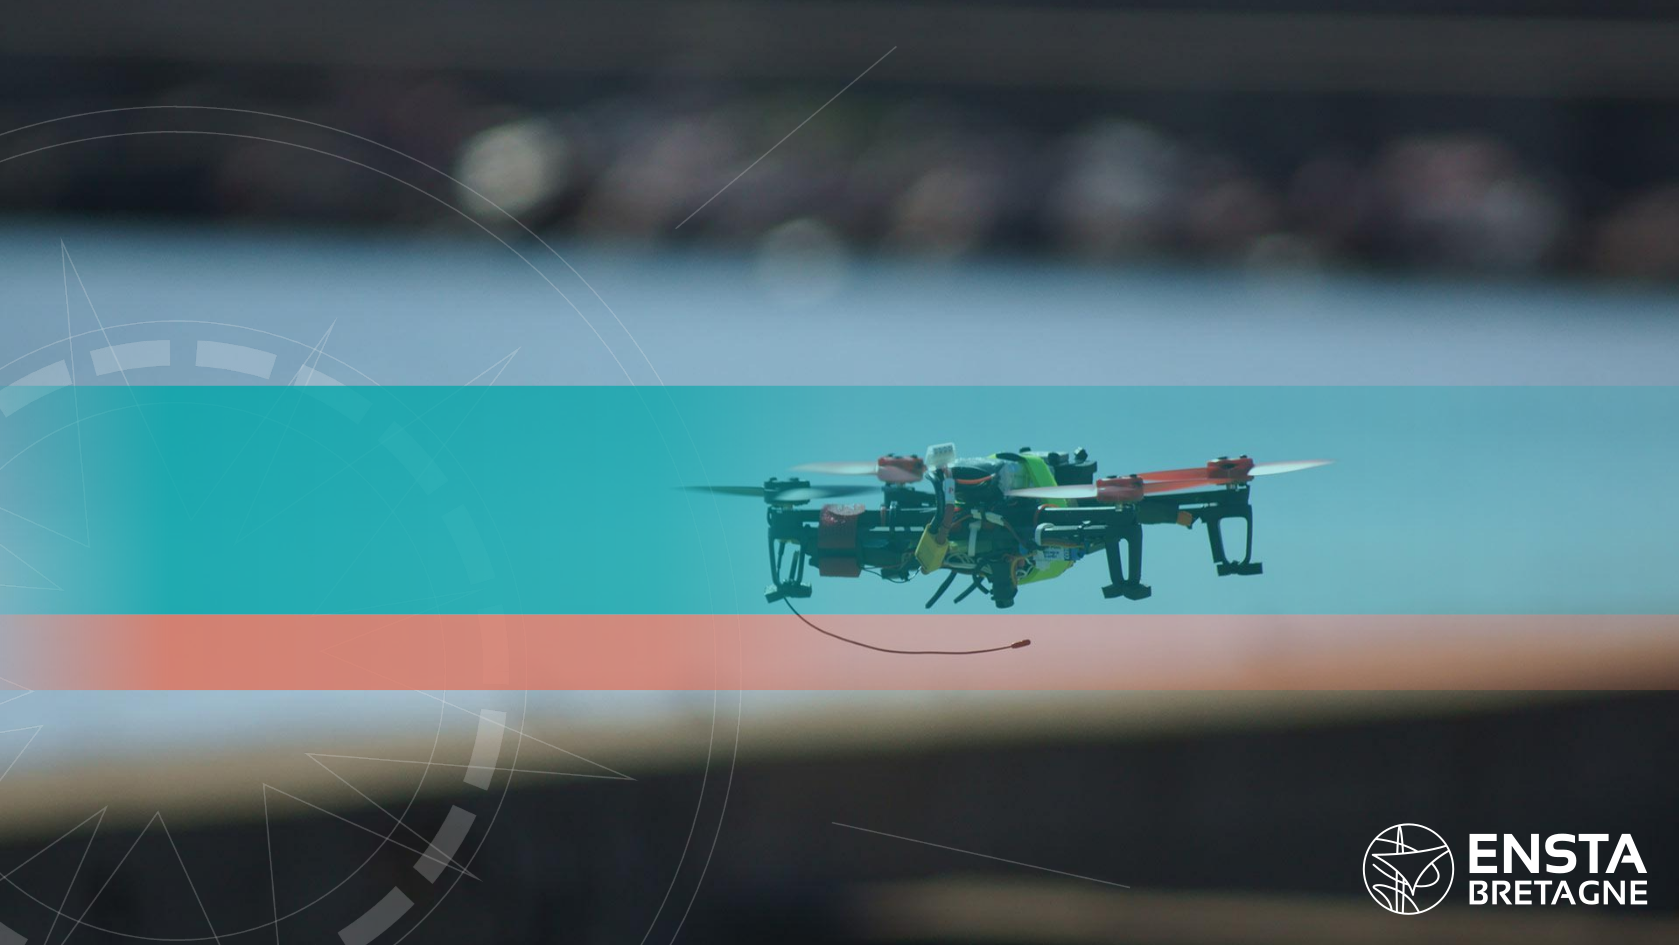
\includegraphics[width=\paperwidth]{images/ensta1.png}}%
	\begin{frame}[plain]
	\maketitle
	\end{frame}
}

\begin{frame}{Frame title}
\begin{exampleblock}{Block title}
Hello world
\end{exampleblock}
\begin{block}{Block title}
Hello world \footfullcite{Feynman1941}
\end{block}
\begin{alertblock}{Block title}
Hello world \cite{Feynman1941}
\end{alertblock}
\end{frame}
\begin{frame}[allowframebreaks]{Lorem ipsum}
\lipsum[1-3]
\end{frame}
\begin{frame}{Image \texttt{textheight}}
\centering
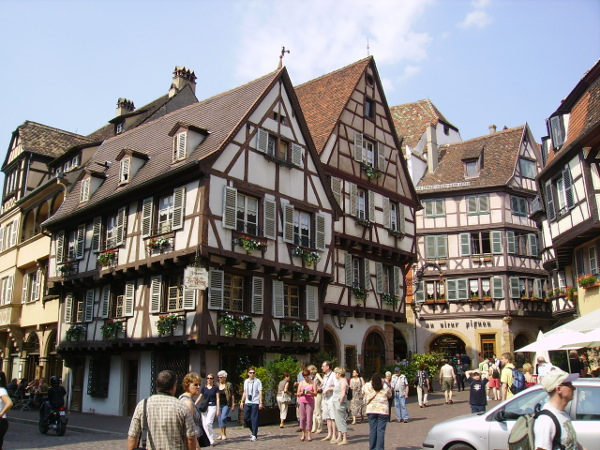
\includegraphics[height=.985\textheight]{images/architecturebretonne_wikipedia.jpg}
\end{frame}
\begin{frame}{Bibliographie}
\printbibliography
\end{frame}
\end{document}